\begin{chapterpage}{Sampling distributions}
  \chaptertitle[30]{Sampling distributions}
  \label{ch_distributions}
  \chaptersection{distributionphat}
\chaptersection{distributionofxbar}


\end{chapterpage}
\renewcommand{\chapterfolder}{ch_distributions}
\index{distribution!normal|(}
\index{normal distribution|}

\chapterintro{In this chapter, we consider what is called the \emph{\hiddenterm{sampling distribution}}, which is a term for describing the distribution of a statistic. For example, if we take a survey of a random sample of the population and compute the proportion of ``yes'' responses, then it's helpful to think of that proportion as being drawn from some distribution.

We will consider sampling distributions for four common statistics: sample proportion, sample mean, difference of sample proportions, and difference of sample means.
In each case, the goal is the same -- to describe the center, spread, and shape of the sampling distribution and determine when normal approximation to the sampling distribution is reasonable.}




%______________________________________________
\section[Sampling distribution of a sample proportion]{Sampling distribution of a sample proportion }
\label{distributionphat}

\sectionintro{
\noindent%
Often, instead of the number of successes in $n$ trials, we are interested in the \emph{proportion} of successes in $n$ trials.  We can use the sampling distribution of a sample proportion to answer questions such as the following:

\begin{itemize}
\item Given a fair coin, what is the probability that in 200 tosses you would get greater than 52\% Tails just by random variation?

\item In a particular state, 48\% support a controversial measure.  When estimating the percent through polling, what is the probability that a random sample of size 200 will mistakenly estimate the percent support to be greater than 50\%?

\end{itemize}


%%
\subsection*{Learning objectives}
\begin{enumerate}
\setlength{\itemsep}{0mm}
\item Understand the concept of a sampling distribution.

\item Describe the center, spread, and shape of the sampling distribution of a sample proportion.

\item Recognize the relationship between the distribution of a sample proportion and the corresponding binomial distribution. 

\item Explain the Central Limit Theorem and what it says about the shape of the sampling distribution of a sample proportion.  

\item Verify appropriate conditions and, if met, carry out normal approximation for a sample proportion or sample count.

\end{enumerate}
}


%%
\subsection[The mean and standard deviation of $\hat{p}$]{The mean and standard deviation of \pmb{$\hat{p}$}}

To answer the two questions posed at the beginning of this section, we investigate the distribution of the sample proportion $\hat{p}$. In the previous section, we saw that the \emph{number} of people with blood type O+ in a random sample of size 40 follows a binomial distribution with $n=40$ and $p=0.35$ that is centered on 14 and has standard deviation 3.0. What does the distribution of the \emph{proportion} of people with blood type O+ in a sample of size 40 look like?  To convert from a count to a proportion, we divide the count (i.e.~number of~yeses) by the sample size, $n = 40$. For example, 8 becomes $8/40 = 0.20$ as a proportion and 11 becomes $11/40 = 0.275$. 

We can find the general formula for the mean (expected value) and standard deviation of a sample proportion $\hat{p}$ using our tools that we've learned so far. To get the sample mean for $\hat{p}$, we divide the binomial mean $\mu_{binomial} = np$ by $n$:
\begin{align*}
\mu_{\hat{p}} = \frac{\mu_{binomial}}{n} = \frac{np}{n} = p
\end{align*}
As one might expect, the sample proportion $\hat{p}$ is centered on the true proportion $p$. Likewise, the standard deviation of $\hat{p}$ is equal to the standard deviation of the binomial distribution divided by $n$:
\begin{align*}
\sigma_{\hat{p}}
	= \frac{\sigma_{binomial}}{n}
	= \frac{\sqrt{np(1-p)}}{n}
	= \sqrt{\frac{p(1-p)}{n}}
\end{align*}

\begin{onebox}{Mean and standard deviation of a sample proportion}
The mean and standard deviation of the sample proportion describe the center and spread of the distribution of all possible sample proportions $\hat{p}$ from a random sample of size $n$ with true population proportion $p$.
\begin{align*}
\mu_{\hat{p}} &= p
	& \sigma_{\hat{p}}&= \sqrt{\frac{p(1-p)}{n}}
	\vspace{1mm}
\end{align*}\end{onebox}

%Because the distribution of $\hat{p}$ is centered at $p$, the sample proportion is said to be an \hiddenterm{unbiased estimator} of $p$.

The standard deviation of a sample proportion, $\sigma_{\hat{p}}$, tells us about the ``typical'' deviation in the sample proportions from the true population proportion.  In analyses, we think of the standard deviation of a sample proportion as describing the uncertainty associated with the estimate $\hat{p}$. That is, $\sigma_{\hat{p}}$ can be thought of as a way to quantify the typical \hiddenterm{error} in our sample estimate $\hat{p}$ of the true proportion $p$. Understanding the variability of statistics such as $\hat{p}$ is a central component in the study of statistics.

In our blood type O+ example, we have $n=40$ and $p=0.35$.  If we look at the distribution of all possible values of a sample proportion for random samples of size 40 from this population, it is centered on $\mu_{\hat{p}} = 0.35$ and has standard deviation $\sigma_{\hat{p}} = \sqrt{\frac{0.35(1-0.35)}{40}}=0.075$.
We see in Figure~\ref{oPositive40prop} that the distribution of proportion of people in a sample of size 40 with blood type O+ is equivalent to the distribution of number of people in a sample with blood type O+ out of 40, but with a change of scale.  Instead of counts along the horizontal axis, we have proportions.  

\begin{figure}[ht]
\centering
\subfigure[]{
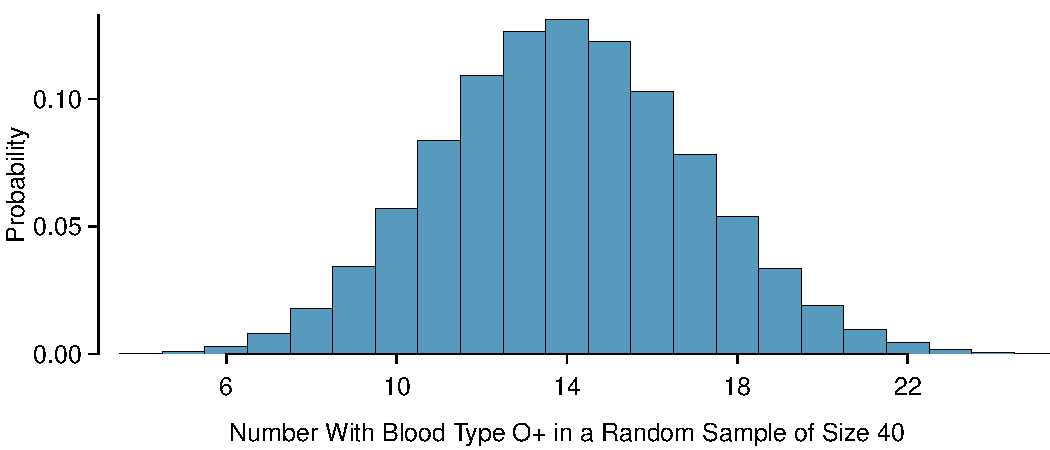
\includegraphics[width=0.475\textwidth]{ch_distributions/figures/oPositive40/oPositive40}
}
\subfigure[]{
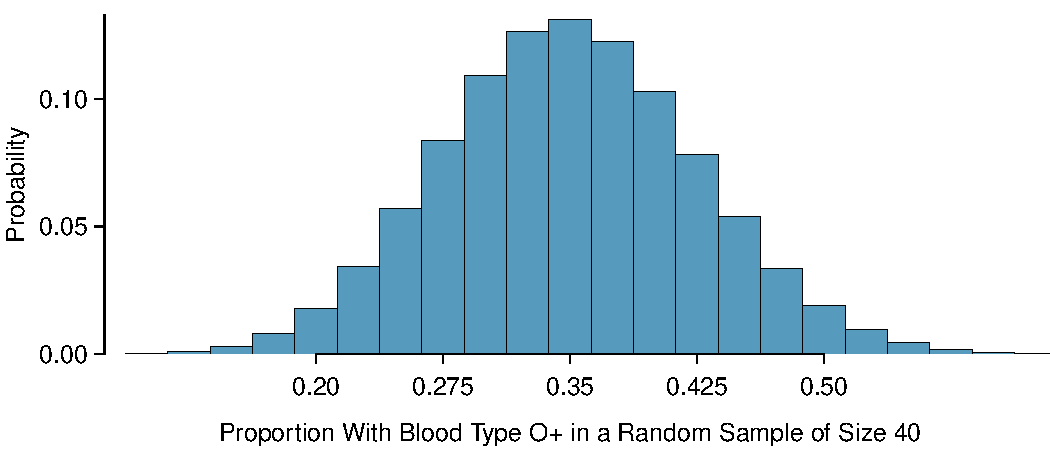
\includegraphics[width=0.475\textwidth]{ch_distributions/figures/oPositive40/oPositive40prop}
}
\caption{Two distributions where $p=0.35$ and $n=40$:  the binomial distribution for the \emph{number} with blood type O+ and the sampling distribution for the \emph{proportion} with blood type O+. }
\label{oPositive40prop}
\end{figure}


%\begin{enumerate}
%\setlength{\itemsep}{0mm}
%\item The average spread of the distribution of all possible values of $\hat{p}$ 
%\item The average \emph{error} of the sample proportion $\hat{p}$, that~is, the average deviation between a particular sample $\hat{p}$ and the true population $p$. 
%\end{enumerate}

\begin{examplewrap}
\begin{nexample}{If the proportion of people in the county with blood type O+ is really 35\%, find and interpret the mean and standard deviation of the sample proportion for a random sample of size 400.}
The mean of the distribution of the sample proportion is the population proportion: 0.35. That is, the distribution of all possible values for the sample proportion is centered on 0.35.  In other words, if we took many, many samples and calculated $\hat{p}$, these values would average out to $0.35$.  

The standard deviation of $\hat{p}$ is described by the standard deviation for the proportion:
\begin{align*}
\sigma_{\hat{p}}
	= \sqrt{\frac{p(1-p)}{n}}
	= \sqrt{\frac{0.35(0.65)}{400}}
	= 0.024
\end{align*}
The sample proportion will typically be about 0.024 or 2.4\% away from the true proportion of $p = 0.35$. We'll become more rigorous about quantifying how close $\hat{p}$ will tend to be to $p$ in Chapter~\ref{foundationsForInference}.
\end{nexample}
\end{examplewrap}


\D{\newpage}

\subsection{Central Limit Theorem}

The distribution in
Figure~\ref{oPositive40prop} looks an awful lot like
a normal distribution. That is no anomaly; it~is the result
of a general principle called the
\index{Central Limit Theorem!proportion|textbf}
\term{Central Limit Theorem}.

\begin{onebox}{Central Limit Theorem and the success-failure condition}
  When observations are independent and the sample size is
  sufficiently large, the sample proportion $\hat{p}$ will tend
  to follow a normal distribution with the following mean and
  standard deviation:%\footnotemark{}
  \begin{align*}
    \mu_{\hat{p}} &= p
    &\sigma_{\hat{p}} &= \sqrt{\frac{p (1 - p)}{n}}
  \end{align*}
  In order for the Central Limit Theorem to hold,
  the sample size is typically considered sufficiently large
  when $np \geq 10$ and $n(1-p) \geq 10$, which is called the
  \term{success-failure condition}.
\end{onebox}


The Central Limit Theorem is incredibly important, and it provides
a foundation for much of statistics.
As we begin applying
the Central Limit Theorem, be mindful of the two
technical conditions:
the observations must be independent, and the sample size must
be sufficiently large such that $np \geq 10$ and $n(1-p) \geq 10$.

\begin{onebox}{How to verify sample observations are independent}
  If the observations are from a random process such as tossing a coin, then they are independent.\stdvspace{}

  If the observations are from a random sample with replacement,
  then they are independent.\stdvspace{}

  If the observations are from a simple random sample (without replacement), we can treat them as independent if the sample size is less than 10\% of the population size.\stdvspace{}

  If a sample is from a seemingly random process,
  e.g. an occasional error on an assembly line,
  checking independence is more difficult. In~this case,
  use your best judgement.
\end{onebox}

When the sample exceeds 10\% of the population size,
the methods we discuss tend to overestimate the sampling error
slightly versus what we would get using more advanced
methods.\footnote{For example, we could use what's called the
  \term{finite population correction factor}:
  if the sample is of size $n$ and the population size is $N$,
  then we can multiple the typical standard deviation formula by
  $\sqrt{\frac{N-n}{N-1}}$
  to obtain a smaller, more precise estimate of the
  actual standard deviation.
  When $n < 0.1 \times N$, this correction factor is relatively close to 1.}


An interesting question to answer is, \emph{what happens when
$np < 10$ or $n(1-p) < 10$}? We can simulate drawing samples of different sizes where,
say, the true proportion is $p = 0.25$.
Here's a sample of size~10:
\begin{center}
% paste(sample(c("yes", "no"), 10, TRUE, c(.25, .75)), collapse = ", ")
no, no, yes, yes, no, no, no, no, no, no
\end{center}
In this sample, we observe a sample proportion of yeses
of $\hat{p} = \frac{2}{10} = 0.2$. We can simulate many such
proportions to understand the sampling distribution of
$\hat{p}$ when $n = 10$ and $p = 0.25$, which we've plotted
in Figure~\ref{sampling_10_prop_25p}
alongside a normal distribution with the
same mean and variability.
These distributions have a number of imprrtant differences.

\begin{figure}[h]
   \centering
   \Figure{0.97}{sampling_10_prop_25p}
   \caption{Left: simulations of $\hat{p}$ when the sample size
       is $n = 10$ and the population proportion is $p = 0.25$.
       Right: a normal distribution with the same mean (0.25)
       and standard deviation (0.137).}
   \label{sampling_10_prop_25p}
\end{figure}

\begin{figure}
   \centering
   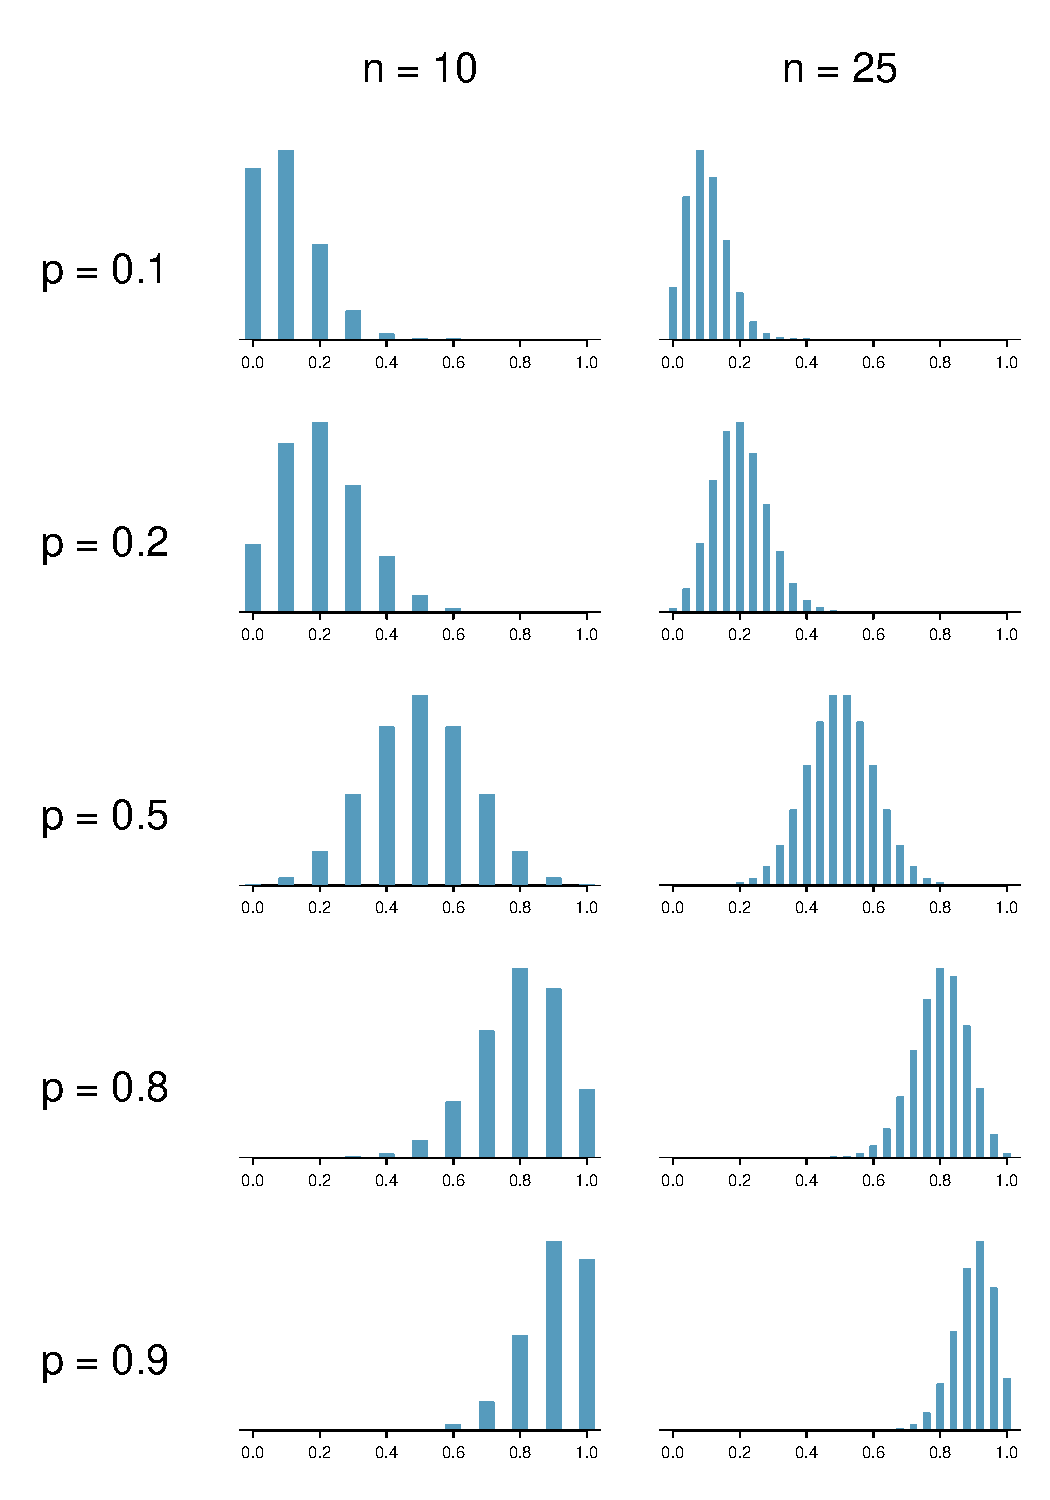
\includegraphics[width=\textwidth]{ch_distributions/figures/clt_prop_grid/clt_prop_grid_1}
   \caption{Sampling distributions for several scenarios
       of $p$ and $n$. \\
       Rows: $p = 0.10$, $p = 0.20$, $p = 0.50$,
       $p = 0.80$, and $p = 0.90$. \\
       Columns: $n = 10$ and $n = 25$.}
   \label{clt_prop_grid_1}
\end{figure}

\begin{figure}
   \centering
   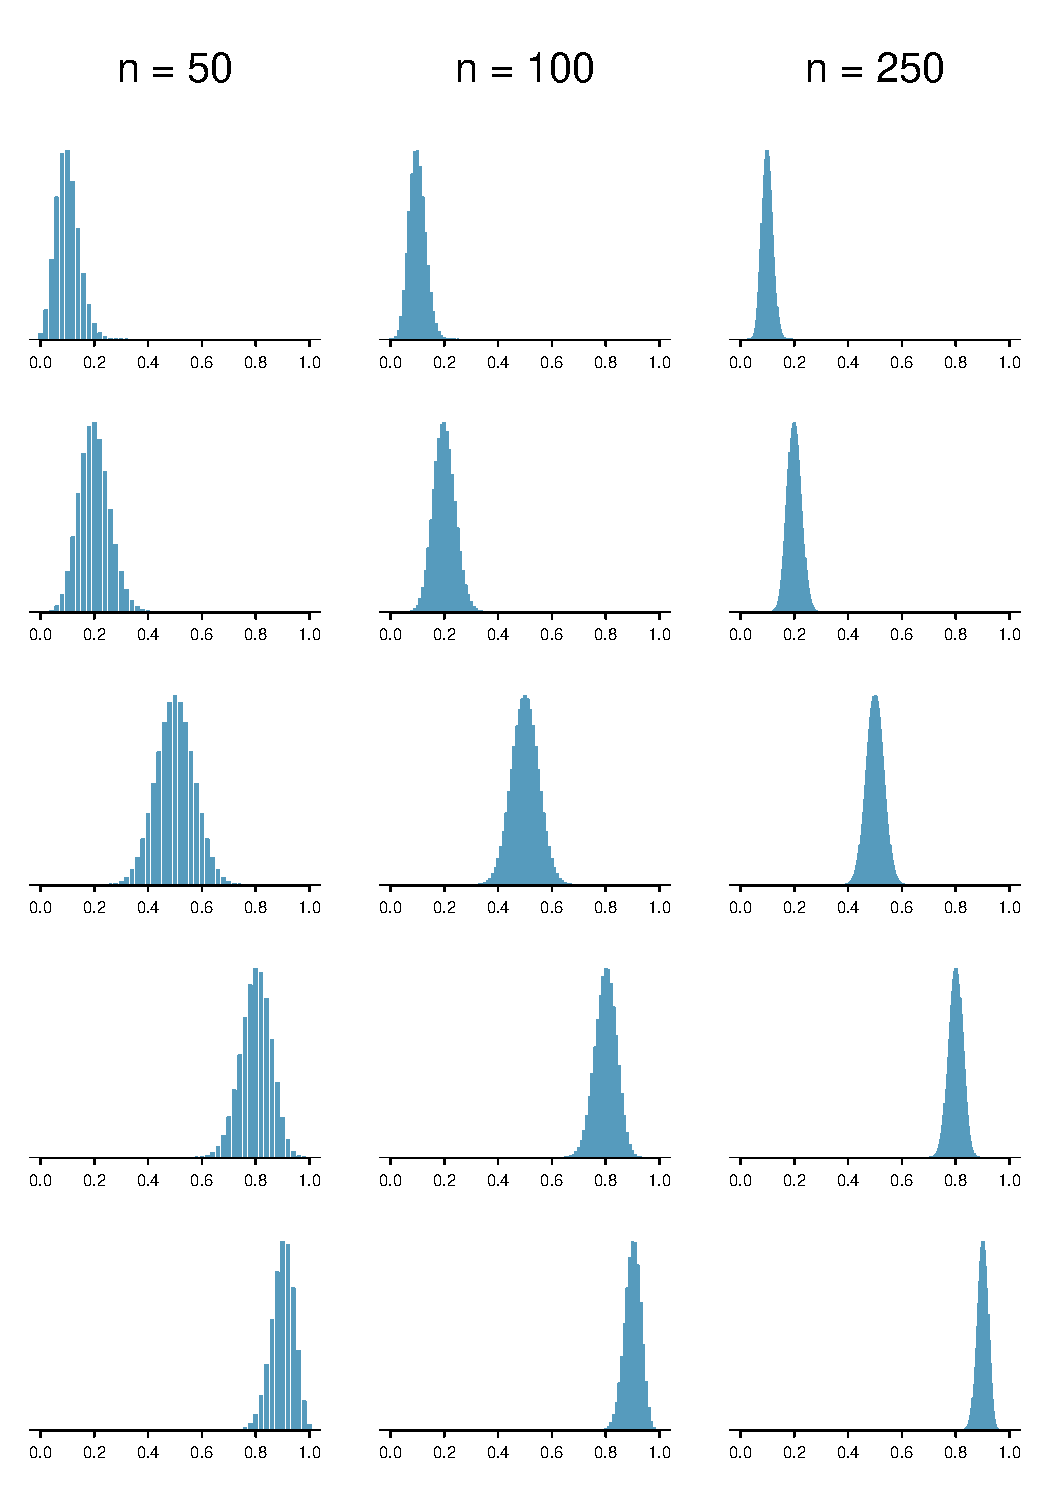
\includegraphics[width=\textwidth]{ch_distributions/figures/clt_prop_grid/clt_prop_grid_2}
   \caption{Sampling distributions for several scenarios
       of $p$ and $n$. \\
       Rows: $p = 0.10$, $p = 0.20$, $p = 0.50$,
       $p = 0.80$, and $p = 0.90$. \\
       Columns: $n = 50$, $n = 100$, and $n = 250$.}
   \label{clt_prop_grid_2}
\end{figure}

\begin{center}
\begin{tabular}{lccc}
\hline
    &  Unimodal?  &  Smooth?  &  Symmetric? \\
\hline
Normal: $N(0.25, 0.14)$  &
    \highlightO{Yes}  &
    \highlightO{Yes}  &
    \highlightO{Yes} \\
$n = 10$, $p = 0.25$  &
    \highlightO{Yes}  &
    \highlightT{No}  &
    \highlightT{No} \\
\hline
\end{tabular}
\end{center}
Notice that the success-failure condition
was not satisfied when $n = 10$ and $p = 0.25$:
\begin{align*}
n p = 10 \times 0.25 = 2.5 &&
    n (1 - p) = 10 \times 0.75 = 7.5
\end{align*}
This single sampling distribution does not show that
the success-failure condition is the perfect guideline,
but we have found that the guideline did correctly
identify that a normal distribution might not be appropriate.

We can complete several additional simulations,
shown in
Figures~\ref{clt_prop_grid_1}
and~\ref{clt_prop_grid_2},
and we can see some trends:
\begin{enumerate}
\item When either $np$ or $n(1 - p)$ is small, the
    distribution is more \term{discrete},
    i.e. \emph{not continuous}.
\item When $np$ or $n(1-p)$ is smaller than~10,
    the skew in the distribution is more noteworthy.
\item The larger both $np$ \emph{and} $n(1 - p)$,
    the more normal the distribution.
    This may be a little harder to see for the larger
    sample size in these plots as the variability
    also becomes much smaller.
\item When $np$ and $n(1 - p)$ are both very large,
    the distribution's discreteness is hardly evident,
    and the distribution looks much more
    like a normal distribution.
\end{enumerate}


\noindent So far we've only focused on the skew and discreteness
of the distributions.
We haven't considered how the mean and standard error
of the distributions change.
Take a moment to look back at the graphs,
and pay attention to three things:
\begin{enumerate}
\item The centers of the distribution are always at
    the population proportion, $p$, that was used to
    generate the simulation. Because the sampling
    distribution of $\hat{p}$ is always centered at
    the population parameter $p$, it means the sample
    proportion $\hat{p}$ is \term{unbiased} when
    the data are independent and drawn from such
    a population.
\item For a particular population proportion $p$,
    the variability in the sampling distribution
    decreases as the sample size~$n$ becomes larger.
    This will likely align with your intuition:
    an estimate based on a larger sample size will
    tend to be more accurate.
\item For a particular sample size, the variability
    will be largest when $p = 0.5$. The differences
    may be a little subtle, so take a close look.
    This reflects the role of the proportion
    $p$ in the standard error formula:
    $SE = \sqrt{\frac{p (1 - p)}{n}}$.
    The standard error is largest when $p = 0.5$.
\end{enumerate}

At no point will the distribution of $\hat{p}$ look
\emph{perfectly} normal, since $\hat{p}$ will always
be take discrete values ($x / n$).
It is always a matter of degree, and we will use
the standard success-failure condition with minimums
of 10 for $np$ and $n (1 - p)$ as our guideline
within this~book.

\begin{onebox}{Three important facts about the distribution of a sample proportion \pmb{$\hat{\MakeLowercase{p}}$}}
When the observations can be considered independent, such as from a random sample of less than 10\% of the population, the distribution of the sample proportion can be described as follows.\begin{enumerate}
\setlength{\itemsep}{0mm}
\item CENTER:  The mean of a sample proportion is $p$.
\item SPREAD:  The SD of a sample proportion is $\sqrt{\frac{p(1-p)}{n}}$.
\item SHAPE:  When $np \geq 10$ and $n(1-p) \geq 10$, the sample proportion closely follows a normal distribution. 
\end{enumerate}\end{onebox}

Using these facts, we can now answer the question posed at the beginning of this section.



%%
\subsection[Normal approximation for the distribution of $\hat{p}$]{Normal approximation for the distribution of \pmb{$\hat{p}$}}

\begin{examplewrap}
\begin{nexample}{Find the probability that less than 30\% of a random sample of 400 people will be blood type O+ if the population proportion is 35\%.}
In the previous section we verified that the observations can be treated as independent and that $np$ and $n(1-p)$ are at least 10. The mean of the sample proportion is 0.35 and the standard deviation for the sample proportion is given by $\sqrt{\frac{0.35(1-0.35)}{400}}=0.024$. We can find a Z-score and use normal approximation to estimate the probability:
\begin{align*}
Z &= \frac{\hat{p} - \mu_{\hat{p}}}{\sigma_{\hat{p}}} = \frac{0.30 - 0.35}{0.024} = -2.1 \\
P(&Z < -2.1) = 0.0179
\end{align*}
We leave it to the reader to construct a figure for this example.
\label{smokers}
\end{nexample}
\end{examplewrap}


\begin{examplewrap}
\begin{nexample}{The probability 0.0179 is the same probability we calculated when we found the probability of getting fewer than 120 with blood type O+ out of 400! Why is this?}
Notice that $120/400=0.30$. Using the binomial distribution to find the probability of fewer than 120 with blood type O+ in the sample is equivalent to using the distribution of $\hat{p}$ to find the probability of a sample proportion less than 0.30.
\end{nexample}
\end{examplewrap}


\begin{exercisewrap}
\begin{nexercise}Given a population that is 50\% male, what is the probability that a random sample of size 200 would have greater than 55\% males?  Remember to verify that conditions for normal approximation are met.\footnotemark
\end{nexercise}
\end{exercisewrap}
\footnotetext{First, verify the conditions: There is a random sample, and the sample size is much smaller than the population size, so observations can be considered independent.  Also, $np = 200(0.5) = 100 \ge 10$ and $n(1-p) = 200 (0.5) = 100 \ge 10$, so the normal approximation is reasonable. Next we find the mean and standard deviation of $\hat{p}$:
\begin{align*}
\mu_{\hat{p}} &= p = 0.50
	& \sigma_{\hat{p}} &= \sqrt{\frac{p(1-p)}{n}}
		= \sqrt{\frac{0.5(0.5)}{200}}
		= 0.0354
\end{align*}
Then we find a Z-score and find the upper tail of the normal distribution:
\begin{align*}
Z = \frac{\hat{p} - \mu_{\hat{p}}}{\sigma_{\hat{p}}} = \frac{0.55 - 0.5}{0.0354} = 1.412
\qquad \rightarrow \qquad
P(Z > 1.412) = 0.07
\end{align*}
The probability of getting a sample proportion greater than 55\% is about 0.07.}


\D{\newpage}

%%
\subsection*{Section summary}

\begin{itemize}
\item A \term{Z-score} represents the number of standard deviations a value in a data set is above or below the mean.  To calculate a \mbox{Z-score} use: $Z = \frac{x-\text{mean}}{SD}$.  

\item The standard deviation of $\hat{p}$ describes the typical error or distance of the sample proportion from the population proportion.  It also tells us how much the sample proportion is likely to vary from one random sample to another.  


\item The sampling distribution of the sample proportion $\hat{p}$ for a random sample of size $n$ is identical to the binomial distribution with parameters $n$ and $p$, but with a change of scale, i.e. different mean and different SD, but same shape.

\item The same \term{success-failure condition} for the binomial distribution holds for a sample proportion $\hat{p}$.

\item Three important facts about the sampling distribution of the sample proportion $\hat{p}$, where the observations can be considered independent:
\begin{itemize}\vspace{-1mm}
\item The mean of a sample proportion is denoted by $\mu_{\hat{p}}$, and it is equal to $p$.  (\textit{center})
\item The SD of a sample proportion is denoted by $\sigma_{\hat{p}}$, and it is equal to $\sqrt{\frac{p(1-p)}{n}}$.  (\textit{spread})
\item When $np\ge 10$ and $n(1-p)\ge 10$, the distribution of the sample proportion will be approximately normal.   (\textit{shape})
\end{itemize}

\item We use these properties when solving the following type of \term{normal approximation} problems involving a sample proportion.  
\emph{Find the probability of getting more / less than \_\_\% yeses in a sample of size $n$}.
\begin{enumerate}\vspace{-1mm}
\setlength{\itemsep}{0mm}
\item Identify $n$ and $p$. Verify than observations can be treated as independent and that $np\ge 10$ and $n(1-p)\ge 10$, which implies that normal approximation is reasonable. 
\item Calculate the Z-score.  Use $\mu_{\hat{p}} = p$ and $\sigma_{\hat{p}} = \sqrt{\frac{p(1-p)}{n}}$ to standardize the sample proportion.  
\item Find the appropriate area under the normal curve.  \end{enumerate}

\end{itemize}

%%%%%%%%%%Section exercises
{\exercisesheader{}

% 39

\eoce{\qt{Distribution of $\hat{p}$} Suppose the true population proportion were $p = 0.95$. The figure below shows what the distribution of a sample proportion looks like when the sample size is $n = 20$, $n = 100$, and $n = 500$. (a) What does each point (observation) in each of the samples represent? (b) Describe the distribution of the sample proportion, $\hat{p}$. How does the distribution of the sample proportion change as $n$ becomes larger?
\begin{center}
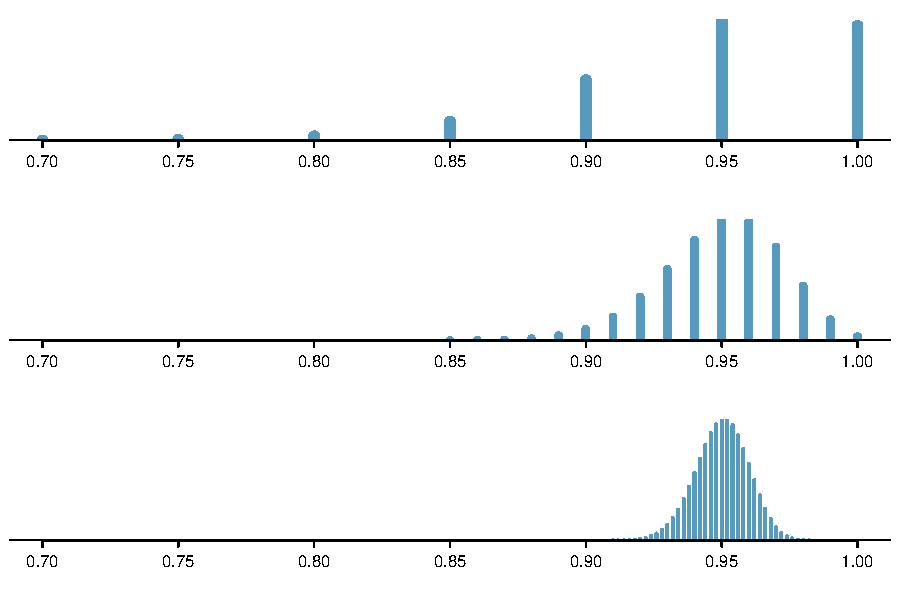
\includegraphics[width=0.85\textwidth]{ch_inference_for_props/figures/eoce/eoce-p-hat-simulations/eoce-p-hat-simulations-p95}
\end{center}}
{}

%40

\eoce{\qt{Distribution of $\hat{p}$} Suppose the true population proportion were $p = 0.5$. The figure below shows what the distribution of a sample proportion looks like when the sample size is $n = 20$, $n = 100$, and $n = 500$. What does each point (observation) in each of the samples represent? Describe how the distribution of the sample proportion, $\hat{p}$, changes as $n$ becomes larger.
\begin{center}
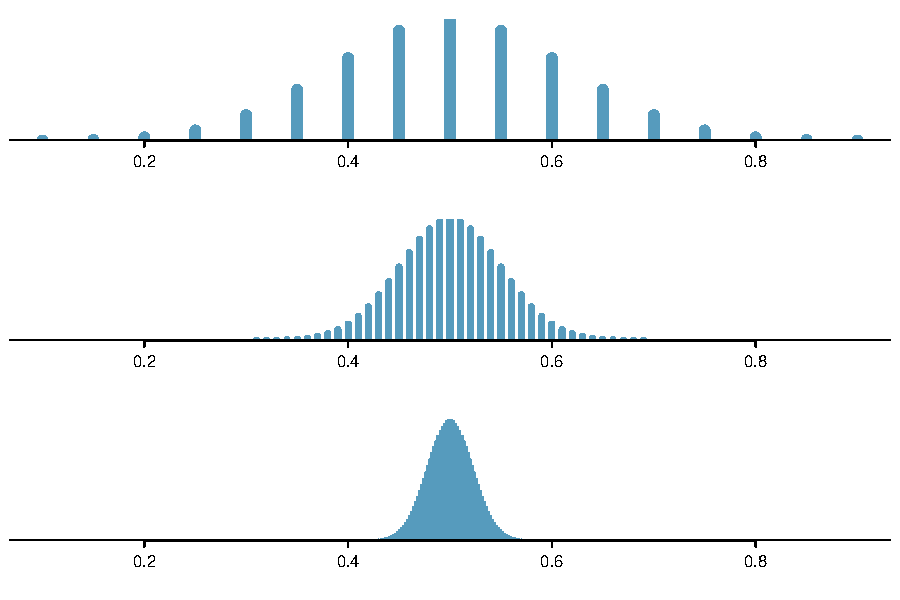
\includegraphics[width=0.85\textwidth]{ch_inference_for_props/figures/eoce/eoce-p-hat-simulations/eoce-p-hat-simulations-p5}
\end{center}}
{}

\D{\newpage}

%41

\eoce{\qt{Distribution of $\hat{p}$} \videohref{ahss_eoce_sol-distribution_of_phat}\ \ Suppose the true population proportion were $p = 0.5$ and a researcher takes a simple random sample of size $n=50$.  
\begin{parts}
\item Find and interpret the standard deviation of the sample proportion $\hat{p}$.  
\item Calculate the probability that the sample proportion will be larger than 0.55 for a random sample of size 50.
\end{parts}
}{}

%42

\eoce{\qt{Distribution of $\hat{p}$} Suppose the true population proportion were $p = 0.6$ and a researcher takes a simple random sample of size $n=50$.  
\begin{parts}
\item Find and interpret the standard deviation of the sample proportion $\hat{p}$. 
\item Calculate the probability that the sample proportion will be larger than 0.65 for a random sample of size 50.
\end{parts}
}{}

% 43

\eoce{\qt{Nearsighted children} \videohref{ahss_eoce_sol-nearsighted_children}\ \ It is believed that nearsightedness affects about 8\% of all children. We are interested in finding the probability that fewer than 12 out of 200 randomly sampled children will be nearsighted.
\begin{parts}
\item Estimate this probability using the normal approximation to the binomial distribution.
\item Estimate this probability using the distribution of the sample proportion.
\item How do your answers from parts (a) and (b) compare?
\end{parts}
}{}


% 44
\eoce{\qt{Social network use} The Pew Research Center estimates that as of January 2014, 89\% of 18-29 year olds in the United States use social networking sites.\footfullcite{data:pewsocialnetwork:2014} Calculate the probability that at least 95\% of 500 randomly sampled 18-29 year olds use social networking sites.
}{}}






%____________________________________
\section[Sampling distribution of a sample mean]{Sampling distribution of a sample mean }
\label{distributionofxbar}

\sectionintro{
\noindent%
If bags of chips are produced with an average weight of 15~oz and a standard deviation of 0.1~oz, what is the probability that the average weight of 30 bags will be within 0.1~oz of the mean?  The answer is not 68\%!
To answer this question we must visualize and understand what is called the \emph{sampling distribution} of a sample mean.


%%
\subsection*{Learning objectives}
\begin{enumerate}
\setlength{\itemsep}{0mm}

\item Describe the center, spread, and shape of the sampling distribution of a sample mean.


\item Distinguish between the standard deviation of a population and the standard deviation of a sampling distribution.

\item Explain the content and importance of the Central Limit Theorem.

\item Identify and explain the conditions for using normal approximation involving a sample mean.

\item Check the appropriate conditions and, when met, carry out normal approximation involving a sample mean or sample sum.

\end{enumerate}
}


%%
\subsection[The mean and standard deviation of $\bar{x}$]{The mean and standard deviation of $\pmb{\bar{x}}$}


In this section we consider a data set called \data{run17}, which represents all 19,961 runners who finished the 2017 Cherry Blossom 10 mile run in Washington, DC.\footnote{\oiRedirect{textbook-cherryblossom_org}{www.cherryblossom.org}} Part of this data set is shown in Figure~\ref{run17DF}, and the variables are described in Figure~\ref{run17Variables}.

\begin{figure}[h]
\centering
\begin{tabular}{rrrrr}
  \hline
ID & time & age & gender & state \\ 
  \hline
1 & 92.25 & 38.00 & M & MD \\ 
2 & 106.35 & 33.00 & M & DC \\ 
%3 & 89.33 & 55.00 & F & VA \\ 
%4 & 113.50 & 24.00 & F & VA \\ 
$\vdots$ & $\vdots$ & $\vdots$ & $\vdots$ & $\vdots$ \\
16923 & 122.87 & 37.00 & F & VA \\ 
16924 & 93.30 & 27.00 & F & DC \\ 
   \hline
\end{tabular}
\caption{Four observations from the \data{run17} data set.}
\label{run17DF}
\end{figure}
% library(openintro); library(xtable); data(run10); xtable(run10[c(1,2,3,4, nrow(run10)-1:0), c("time", "age", "gender", "state")])

\begin{figure}[h]
\centering\small
\begin{tabular}{l p{65mm}}
\hline
{\bf variable} & {\bf description} \\
\hline
\var{time} & Ten mile run time, in minutes \\
\var{age} & Age, in years \\
\var{gender} & Gender (\resp{M} for male, \resp{F} for female) \\
\var{state} & Home state (or country if not from the US) \\
\hline
\end{tabular}
\caption{Variables and their descriptions for the \data{run17} data set.}
\label{run17Variables}
\end{figure}

\index{data!run17samp|(}

\D{\newpage}

These data are special because they include the results for the entire population of runners who finished the 2017 Cherry Blossom Run. We took a simple random sample of this population, which is represented in Figure~\ref{run17sampDF}. A histogram summarizing the time variable in the \data{run17samp} data set is shown in Figure~\ref{run17sampHistograms}.

\begin{figure}[h]
\centering
\begin{tabular}{rrrrr}
  \hline
ID & time & age & gender & state \\ 
  \hline
1983 & 88.31 & 59 & M & MD \\ 
8192 & 100.67 & 32 & M & VA \\ 
%11020 & 109.52 & 33 & F & VA \\ 
  $\vdots$ &   $\vdots$ &   $\vdots$ &   $\vdots$ &   $\vdots$ \\ 
1287 & 89.49 & 26 & M & DC \\ 
   \hline
\end{tabular}
\caption{Three observations for the \data{run17samp} data set, which represents a simple random sample of 100 runners from the 2017 Cherry Blossom Run.}
\label{run17sampDF}
%library(openintro); library(xtable); data(run10); data(run10samp); xtable(run10samp[c(1,2,3,100),])
\end{figure}

% WARNING: This figure is referenced in Section 4.2

\begin{figure}[h]
\centering
\includegraphics[width=0.75\textwidth]{ch_distributions/figures/run17sampHistograms/run17sampHistograms} 
\caption{Histogram of \var{time} for a single sample of size 100. The average of the sample is in the mid-90s and the standard deviation of the sample $s\approx 17$ minutes.
}
\label{run17sampHistograms}
\end{figure}

From the random sample represented in \data{run17samp}, we guessed the average time it takes to run 10 miles is 95.61 minutes. Suppose we take another random sample of 100 individuals and take its mean: 95.30 minutes. Suppose we took another (93.43 minutes) and another (94.16 minutes), and so on. If we do this many many times -- which we can do only because we have the entire population data set -- we can build up a \term{sampling distribution} for the sample mean when the sample size is 100, shown in Figure~\ref{netTime1000SamplingDistribution}.

\begin{figure}[h]
   \centering
   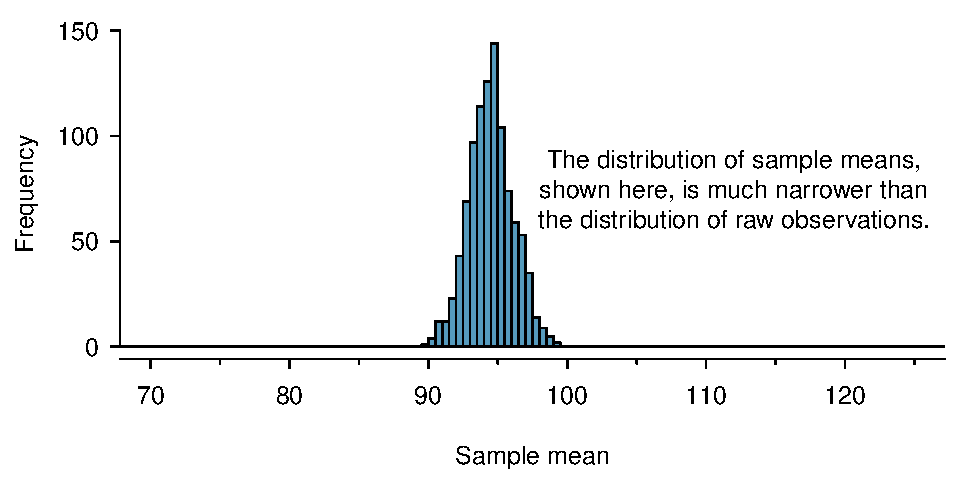
\includegraphics[width=\textwidth]{ch_distributions/figures/netTime1000SamplingDistribution/netTime1000SamplingDistribution}
   \caption{A histogram of 1000 sample means for run time, where the samples are of size $n=100$. This histogram approximates the true sampling distribution of the sample mean, with mean $\mu_{\bar{x}}$ and standard deviation $\sigma_{\bar{x}}$.}
   \label{netTime1000SamplingDistribution}
\end{figure}

\begin{onebox}{Sampling distribution}
The sampling distribution represents the distribution of the point estimates based on samples of a fixed size from a certain population. It is useful to think of a point estimate as being drawn from such a distribution. Understanding the concept of a sampling distribution is central to understanding statistical inference.\end{onebox}


The sampling distribution shown in Figure~\ref{netTime1000SamplingDistribution} is unimodal and approximately symmetric. It is also centered exactly at the true population mean: $\mu=94.52$. Intuitively, this makes sense. The sample mean should be an unbiased estimator of the population mean. Because we are considering the distribution of the sample mean, we will use $\mu_{\bar{x}} = 94.52$ to describe the true mean of this distribution.

\D{\newpage}

We can see that the sample mean has some variability around the population mean, which can be quantified using the standard deviation of this distribution of sample means. The standard deviation of the sample mean tells us how far the typical estimate is away from the actual population mean, 94.52 minutes. It also describes the typical \term{error} of a single estimate, and is denoted by the symbol $\sigma_{\bar{x}}$. 

\begin{onebox}{Standard deviation of an estimate}
The standard deviation associated with an estimate describes the typical error or uncertainty associated with the estimate.\end{onebox}

\begin{examplewrap}
\begin{nexample}{Looking at Figures~\ref{run17sampHistograms} and \ref{netTime1000SamplingDistribution}, we see that the standard deviation of the sample mean with $n=100$ is much smaller than the standard deviation of a single sample. Interpret this statement and explain why it is true.}The variation from one sample mean to another sample mean is much smaller than the variation from one individual to another individual. This makes sense because when we average over 100 values, the large and small values tend to cancel each other out. While many individuals have a time under 90 minutes, it would be unlikely for the \emph{average} of 100 runners to be less than 90 minutes.
\end{nexample}
\end{examplewrap}

\D{\newpage}

\begin{exercisewrap}
\begin{nexercise}
(a) Would you rather use a small sample or a large sample when estimating a parameter? Why? (b) Using your reasoning from (a), would you expect a point estimate based on a small sample to have smaller or larger standard deviation than a point estimate based on a larger sample?\footnotemark
\end{nexercise}
\end{exercisewrap}
\footnotetext{(a) Consider two random samples: one of size 10 and one of size 1000. Individual observations in the small sample are highly influential on the estimate while in larger samples these individual observations would more often average each other out. The larger sample would tend to provide a more accurate estimate. (b) If we think an estimate is better, we probably mean it typically has less error. Based on (a), our intuition suggests that a larger sample size corresponds to a smaller standard deviation.}

When considering how to calculate the standard deviation of a sample mean, there is one problem: there is no obvious way to estimate this from a single sample. However, statistical theory provides a helpful tool to address this issue.

In the sample of 100 runners, the standard deviation of the sample mean is equal to one-tenth of the population standard deviation: $15.93/10 = 1.59$. In other words, the standard deviation of the sample mean based on 100 observations is equal to
\begin{eqnarray*}
SD_{\bar{x}} = \sigma_{\bar{x}} = \frac{\sigma_{x}}{\sqrt{n}} = \frac{15.93}{\sqrt{100}} = 1.59
\end{eqnarray*}
where $\sigma_{x}$ is the standard deviation of the individual observations. This is no coincidence. We can show mathematically that this equation is correct when the observations are independent  using the probability tools of Section~\ref{randomVariablesSection}.

\begin{onebox}{Computing SD for the sample mean}
Given $n$ independent observations from a population with standard deviation $\sigma$, the standard deviation of the sample mean is equal to \vspace{-1mm}
\begin{eqnarray}
SD_{\bar{x}} = \sigma_{\bar{x}} =  \frac{\sigma}{\sqrt{n}}
\label{seOfXBar}
\end{eqnarray}\vspace{-3mm}

A reliable method to ensure sample observations are independent is to conduct a simple random sample consisting of less than 10\% of the population.\index{standard error!single mean}\end{onebox}

\begin{exercisewrap}
\begin{nexercise}
The average of the runners' ages is 35.05 years with a standard deviation of $\sigma = 8.97$. A simple random sample of 100 runners is taken. (a)~What is the standard deviation of the sample mean? (b)~Would you be surprised to get a sample of size 100 with an average of 36~years?\footnotemark\end{nexercise}
\end{exercisewrap}
\footnotetext{(a) Use Equation~(\ref{seOfXBar}) with the population standard deviation to compute the standard deviation of the sample mean: $SD_{\bar{y}} = 8.97/\sqrt{100} = 0.90$ years. (b) It would not be surprising. 36 years is about 1 standard deviation from the true mean of 35.05. Based on the 68, 95 rule, we would get a sample mean at least this far away from the true mean approximately $100\% - 68\% = 32\%$ of the time.}

%library(openintro); library(xtable); data(run10); data(run10samp); mean(run10samp$age); sd(run10samp$age); sd(run10$age, na.rm=TRUE)

\begin{exercisewrap}
\begin{nexercise}
(a) Would you be more trusting of a sample that has 100 observations or 400 observations? (b) We want to show mathematically that our estimate tends to be better when the sample size is larger. If the standard deviation of the individual observations is 10, what is our estimate of the standard deviation of the mean when the sample size is 100? What about when it is 400? (c) Explain how your answer to (b) mathematically justifies your intuition in part~(a).\footnotemark
\end{nexercise}
\end{exercisewrap}
\footnotetext{(a) Extra observations are usually helpful in understanding the population, so a point estimate with 400 observations seems more trustworthy. (b) The standard deviation of the mean when the sample size is 100 is given by $SD_{100} = 10/\sqrt{100} = 1$. For 400: $SD_{400} = 10/\sqrt{400} = 0.5$. The larger sample has a smaller standard deviation of the mean. (c) The standard deviation of the mean of the sample with 400 observations is lower than that of the sample with 100 observations. The standard deviation of $\bar{x}$ describes the typical error, and since it is lower for the larger sample, this mathematically shows the estimate from the larger sample tends to be better -- though it does not guarantee that every large sample will provide a better estimate than a particular small sample.}


\D{\newpage}

%%
\subsection{Examining the Central Limit Theorem}
\label{cltSection}

\index{Central Limit Theorem|(}

In Figure~\ref{netTime1000SamplingDistribution}, the sampling distribution of the sample mean looks approximately normally distributed. Will the sampling distribution of a mean always be nearly normal? To address this question, we will investigate three cases to see roughly when the approximation is reasonable.

We consider three data sets: one from a \emph{uniform} distribution, one from an \emph{exponential} distribution, and the other from a \emph{normal} distribution. These distributions are shown in the top panels of Figure~\ref{cltSimulations}. The uniform distribution is symmetric, and the exponential distribution may be considered as having moderate skew since its right tail is relatively short (few outliers).

\begin{figure}
   \centering
   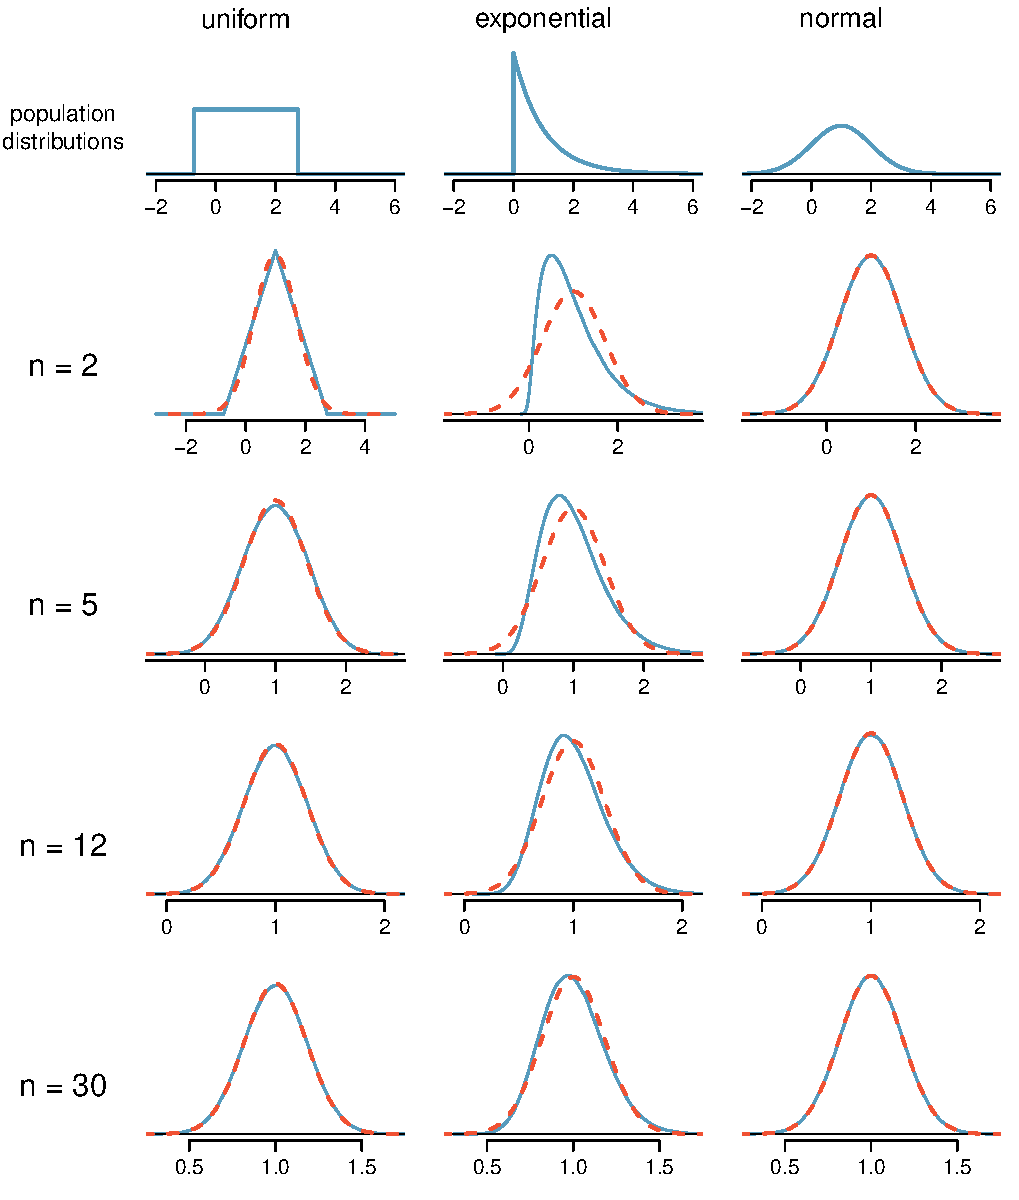
\includegraphics[width=\textwidth]{ch_distributions/figures/cltSimulations/cltSimulations}
   \caption{Sampling distributions for the mean at different sample sizes and for three different distributions. The dashed red lines show normal distributions.}
   \label{cltSimulations}
\end{figure}

The left panel in the $n=2$ row represents the sampling distribution of $\bar{x}$ if it is the sample mean of two observations from the uniform distribution shown. The dashed line represents the closest approximation of the normal distribution. Similarly, the center and right panels of the $n=2$ row represent the respective distributions of $\bar{x}$ for data from exponential and log-normal distributions.

\begin{exercisewrap}
\begin{nexercise}
Examine the distributions in each row of Figure~\ref{cltSimulations}. What do you notice about the sampling distribution of the mean as the sample size, $n$, becomes larger?\footnotemark
\end{nexercise}
\end{exercisewrap}
\footnotetext{The normal approximation becomes better as larger samples are used. However, in the case when the population is normally distributed, the normal distribution of the sample mean is normal for all sample sizes.}

\begin{examplewrap}
\begin{nexample}{In general, would normal approximation for a sample mean be appropriate when the sample size is at least 30?}
Yes, the sampling distributions when $n = 30$ all look very much like the normal distribution.

However, the more non-normal a population distribution, the larger a sample size is necessary for the sampling distribution to look nearly normal.
\end{nexample}
\end{examplewrap}

\begin{onebox}{Determining if the sample mean is normally distributed}
If the population is normal, the sampling distribution of $\bar{x}$ will be normal for any sample size. \\[2mm]
The less normal the population, the larger $n$ needs to be for the sampling distribution of $\bar{x}$ to be nearly normal. However, a good rule of thumb is that for almost all populations, the sampling distribution of $\bar{x}$ will be approximately normal if $n \ge 30$.\end{onebox}

This brings us to the \term{Central Limit Theorem}, the most fundamental theorem in Statistics.

\begin{onebox}{Central Limit Theorem}
When taking a random sample of independent observations from a population with a fixed mean and standard deviation, the distribution of $\bar{x}$ approaches the normal distribution as $n$ increases.\end{onebox}

\D{\newpage}

\begin{examplewrap}
\begin{nexample}{Sometimes we do not know what the population distribution looks like. We have to infer it based on the distribution of a single sample. Figure~\ref{pokerProfitsCanApplyNormalToSampMean} shows a histogram of 20 observations. These represent winnings and losses from 20 consecutive days of a professional poker player. Based on this sample data, can the normal approximation be applied to the distribution of the sample mean?}
We should consider each of the required conditions.
\begin{itemize}
\setlength{\itemsep}{0mm}
\item[(1)] These are referred to as \term{time series data}, because the data arrived in a particular sequence. If the player wins on one day, it may influence how she plays the next. To make the assumption of independence we should perform careful checks on such data.
\item[(2)] The sample size is 20, which is smaller than 30.
\item[(3)] There are two outliers in the data, both quite extreme, which suggests the population may not be normal and instead may be very strongly skewed or have distant outliers. Outliers can play an important role and affect the distribution of the sample mean and the estimate of the standard deviation of the sample mean.
\end{itemize}
Since we should be skeptical of the independence of observations and the extreme upper outliers pose a challenge, we should not use the normal model for the sample mean of these 20 observations. If we can obtain a much larger sample, then the concerns about skew and outliers would no longer apply.
\end{nexample}
\end{examplewrap}

\begin{figure}[ht]
   \centering
   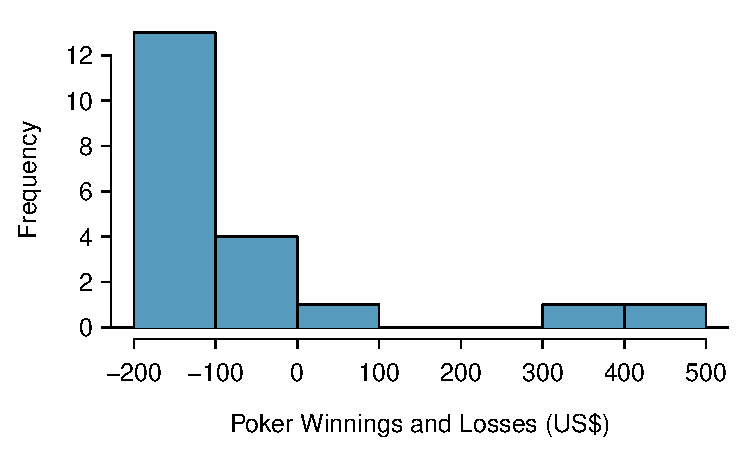
\includegraphics[height=58mm]{ch_distributions/figures/pokerProfitsCanApplyNormalToSampMean/pokerProfitsCanApplyNormalToSampMean}
   \caption{Sample distribution of poker winnings. These data include two very clear outliers. These are problematic when considering the normality of the sample mean. For example, outliers are often an indicator of very strong skew.}
   \label{pokerProfitsCanApplyNormalToSampMean}
\end{figure}

\begin{onebox}{Examine data structure when considering independence}
{Some data sets are collected in such a way that they have a natural underlying structure between observations, e.g. when observations occur consecutively. Be especially cautious about independence assumptions regarding such data sets.}
\end{onebox}

\begin{onebox}{Watch out for strong skew and outliers}
{Strong skew in the population is often identified by the presence of clear outliers in the data. If a data set has prominent outliers, then a larger sample size will be needed for the sampling distribution of $\bar{x}$ to be normal. There are no simple guidelines for what sample size is big enough for each situation. However, we can use the rule of thumb that, in general, an $n$ of at least 30 is sufficient for most cases.}
\index{skew!strongly skewed guideline}
\end{onebox}
\index{Central Limit Theorem|)}


\D{\newpage}

%%
\subsection[Normal approximation for the sampling distribution of $\bar{x}$]{Normal approximation for the sampling distribution of \pmb{$\bar{x}$}}

At the beginning of this chapter, we used normal approximation for populations or for data that had an approximately normal distribution. When appropriate conditions are met, we can also use the normal approximation to estimate probabilities about a sample average. We must remember to verify that the conditions are met and use the mean $\mu_{\bar{x}}$ and standard deviation $\sigma_{\bar{x}}$ for the sampling distribution of the sample average.

\begin{onebox}{Three important facts about the distribution of a sample mean \pmb{\MakeLowercase{$\bar{x}$}}}
When the observations can be considered independent, such as from a random sample of less than 10\% of the population, the distribution of the sample mean can be described as follows.\begin{enumerate}
\setlength{\itemsep}{0mm}
\item The mean of a sample mean is denoted by $\mu_{\bar{x}}$, and it is equal to $\mu$.
\item The SD of a sample mean is denoted by $\sigma_{\bar{x}}$, and it is equal to $\frac{\sigma}{\sqrt{n}}$.
\item When the population is normal or when $n\ge 30$, the sample mean closely follows a normal distribution. 
\end{enumerate}\end{onebox}

\begin{examplewrap}
\begin{nexample}{
In the 2017 Cherry Blossom 10 mile run, the average time for all of the runners is 94.52 minutes with a standard deviation of 8.97 minutes. The distribution of run times is approximately normal. Find the probabiliy that a randomly selected runner completes the run in less than 90 minutes.}Because the distribution of run times is approximately normal, we can use normal approximation.
\begin{align*}
&Z = \frac{x - \mu}{\sigma}=\frac{90-94.52}{8.97}=-0.504 \\
&P(Z < -0.504) = 0.3072
\end{align*}
There is a 30.72\% probability that a randomly selected runner will complete the run in less than 90~minutes.
\end{nexample}
\end{examplewrap}

\begin{examplewrap}
\begin{nexample}{
Find the probabiliy that the average of 20 runners is less than 90~minutes.}
Here, $n=20<30$, but the distribution of the population, that~is, the distribution of run times is stated to be approximately normal. Because of this, the sampling distribution will be normal for any sample size.
\begin{align*}
&\sigma_{\bar{x}}=\frac{\sigma}{\sqrt{n}}=\frac{8.97}{\sqrt{20}}=2.01 \\
&Z = \frac{\bar{x} - \mu_{\bar{x}}}{\sigma_{\bar{x}}}=\frac{90-94.52}{2.01}=-2.25\\
&P(Z < -2.25) = 0.0123
\end{align*}
There is a 1.23\% probability that the average run time of 20 randomly selected runners will be less than 90~minutes.
\end{nexample}
\end{examplewrap}

\D{\newpage}

\begin{examplewrap}
\begin{nexample}{
The average of all the runners' ages is 35.05 years with a standard deviation of $\sigma = 8.97$. The distribution of age is somewhat skewed. What is the probability that a randomly selected runner is older than 37 years?}Because the distribution of age is skewed and is not normal, we cannot use normal approximation for this problem. In order to answer this question, we would need to look at all of the data.
\end{nexample}
\end{examplewrap}

\begin{exercisewrap}
\begin{nexercise}
What is the probability that the average of 50 randomly selected runners is greater than 37 years?\footnotemark
\end{nexercise}
\end{exercisewrap}
\footnotetext{Because $n=50\ge 30$, the sampling distribution of the mean is approximately normal, so we can use normal approximation for this problem. The mean is given as 35.05 years.
\begin{align*}
&\sigma_{\bar{x}}
	= \frac{\sigma}{\sqrt{n}}
	= \frac{8.97}{\sqrt{50}}=1.27
&&z=\frac{\bar{x}-\mu_{\bar{x}}}{\sigma_{\bar{x}}} = \frac{37-35.05}{1.27}=1.535
&&P(Z > 1.535) = 0.062
\end{align*}
There is a 6.2\% chance that the average age of 50 runners will be greater than 37.} 

\begin{onebox}{Remember to divide by $\pmb{\sqrt{\MakeLowercase{n}}}$}
When finding the probability that an \emph{average} or mean is greater or less than a particular value, remember to divide the standard deviation of the population by $\sqrt{n}$ to calculate the correct~SD.\end{onebox}


\D{\newpage}

%%
\subsection*{Section summary}

\begin{itemize}
\item The symbol $\bar{x}$ denotes the sample average.  $\bar{x}$ for any particular sample is a number.  However, $\bar{x}$ can vary from sample to sample.  The distribution of all possible values of $\bar{x}$ for repeated samples of a fixed size from a certain population is called the \term{sampling distribution} of $\bar{x}$.

\item The standard deviation of $\bar{x}$ describes the typical error or distance of the sample mean from the population mean.  It also tells us how much the sample mean is likely to vary from one random sample to another.  

\item The standard deviation of $\bar{x}$ will be \textit{smaller} than the standard deviation of the population by a factor of $\sqrt{n}$.  The larger the sample, the better the estimate tends to be.

\item Consider taking a simple random sample from a population with a fixed mean and standard deviation.  The \term{Central Limit Theorem} ensures that regardless of the shape of the original population, as the sample size increases, the distribution of the sample average $\bar{x}$ becomes more normal.  

\item Three important facts about the sampling distribution of the sample average $\bar{x}$ where the observations can be treated as independent:
\begin{itemize}\vspace{-1mm}
\setlength{\itemsep}{0mm}
\item The mean of a sample mean is denoted by $\mu_{\bar{x}}$, and it is equal to $\mu$. (\textit{center})
\item The SD of a sample mean is denoted by $\sigma_{\bar{x}}$, and it is equal to $\frac{\sigma}{\sqrt{n}}$.  (\textit{spread})
\item When the population is normal or when $n\ge 30$, the sample mean closely follows a normal distribution.   (\textit{shape})
\end{itemize}

\item These facts are used when solving the following two types of \textbf{normal approximation} problems involving a \emph{sample mean} or a \emph{sample sum}.  
\begin{itemize}
\item[A:] \textit{Find the probability that a sample average will be greater/less than a certain value}.
\begin{enumerate}\vspace{-1mm}
\setlength{\itemsep}{0mm}
\item Verify that the observations can be treated as independent and that either the population is approximately normal or $n \ge 30$.
\item Calculate the Z-score.  Use $\mu_{\bar{x}}=\mu$ and $\sigma_{\bar{x}}=\frac{\sigma}{\sqrt{n}}$ to standardize the sample average.  
\item Find the appropriate area under the normal curve.  
\end{enumerate}

\item[B:] \textit{Find the probability that a sample sum/total will be greater/less than a certain value}.
\begin{enumerate}\vspace{-1mm}
\setlength{\itemsep}{0mm}
\item Convert the sample sum into a sample average, using $\bar{x} = \frac{sum}{n}$.  
\item Do steps 1-3 from Part A above.
\end{enumerate}
\end{itemize}
\end{itemize}

%%%%%%%%%%Section exercises
{\exercisesheader{}

% 7 - ages_pennies_1

\eoce{\qt{Ages of pennies, Part I \label{ages_pennies_1}} The histogram below shows the distribution of ages of pennies at a bank. 

\noindent\begin{minipage}[c]{0.54\textwidth}
\begin{parts}
\item Describe the distribution.
\item Sampling distributions for means from simple random samples of 5, 30, and 100 pennies is shown in the histograms below. Describe the shapes of these distributions and comment on whether they look like what you would expect to see based on the Central Limit Theorem.
\end{parts}
\end{minipage}
\begin{minipage}[c]{0.44\textwidth}
\begin{center}
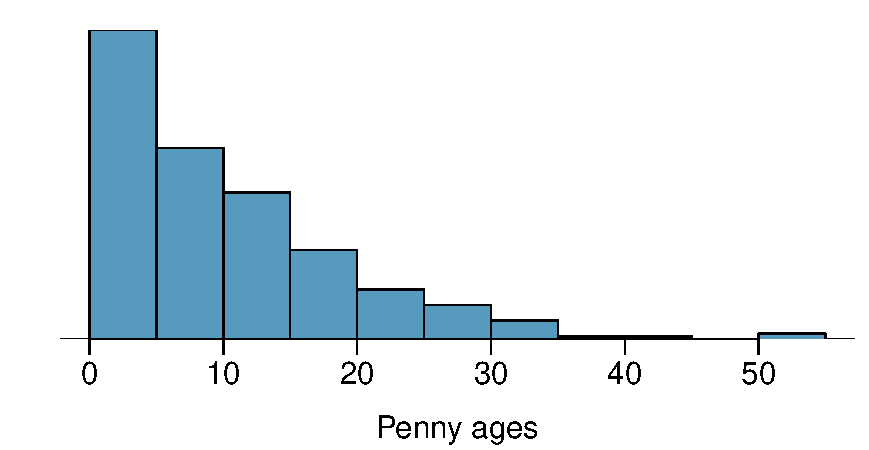
\includegraphics[width=\textwidth]{ch_distributions/figures/eoce/ages_pennies_1/penniesAges_pop} 
\end{center}
\end{minipage}\vspace{-1mm}
\begin{center}
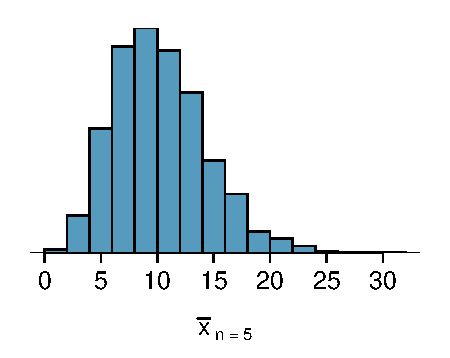
\includegraphics[width=0.325\textwidth]{ch_distributions/figures/eoce/ages_pennies_1/penniesAges_n5} 
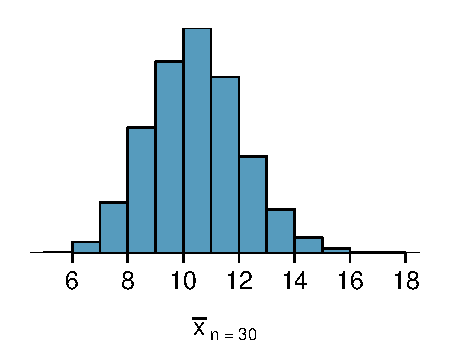
\includegraphics[width= 0.325\textwidth]{ch_distributions/figures/eoce/ages_pennies_1/penniesAges_n30} 
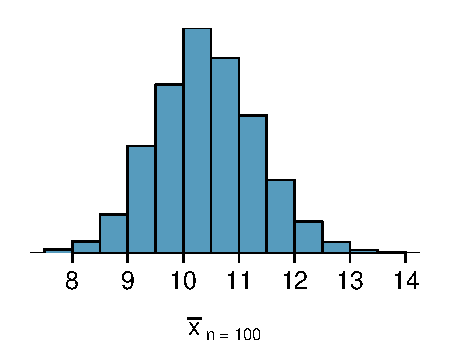
\includegraphics[width= 0.325\textwidth]{ch_distributions/figures/eoce/ages_pennies_1/penniesAges_n100} 
\end{center}
}{}

% 8 - ages_pennies_2

\eoce{\qt{Ages of pennies, Part II\label{ages_pennies_2}} The mean age of the pennies from Exercise~\ref{ages_pennies_1} is 10.44 years with a standard deviation of 9.2 years. Using the Central Limit Theorem, calculate the means and standard deviations of the distribution of the mean from random samples of size 5, 30, and 100. Comment on whether the sampling distributions shown in Exercise~\ref{ages_pennies_1} agree with the values you compute.
}{}

% 9 - housing_prices

\eoce{\qt{Housing prices\label{housing_prices}} \videosolution{ahss_eoce_sol-housing_prices} A housing survey was conducted to 
determine the price of a typical home in Topanga, CA. The mean price of a house 
was roughly \$1.3 million with a standard deviation of \$300,000. There were no 
houses listed below \$600,000 but a few houses above \$3 million.
\begin{parts}
\item Is the distribution of housing prices in Topanga symmetric, right skewed, 
or left skewed? \textit{Hint:} Sketch the distribution.
\item Would you expect most houses in Topanga to cost more or less than \$1.3 
million?
\item Can we estimate the probability that a randomly chosen house in Topanga 
costs more than \$1.4 million using the normal distribution?
\item What is the probability that the mean of 60 randomly chosen houses in 
Topanga is more than \$1.4 million?
\item How would doubling the sample size affect the standard deviation of the 
mean?
\end{parts}
}{}

% 10 - stats_final_scores

\eoce{\qt{Stats final scores\label{stats_final_scores}} Each year about 1500 students 
take the introductory statistics course at a large university. This year scores 
on the final exam are distributed with a median of 74 points, a mean of 70 
points, and a standard deviation of 10 points. There are no students who scored 
above 100 (the maximum score attainable on the final) but a few students scored 
below 20 points.
\begin{parts}
\item Is the distribution of scores on this final exam symmetric, right skewed, 
or left skewed?
\item Would you expect most students to have scored above or below 70 points?
\item Can we calculate the probability that a randomly chosen student scored 
above 75 using the normal distribution?
\item What is the probability that the average score for a random sample of 40 
students is above 75?
\item How would cutting the sample size in half affect the standard deviation of 
the mean?
\end{parts}
}{}

% 11 - identify_dist_symm_pop

\eoce{\qt{Identify distributions, Part I\label{identify_dist_symm_pop}} Four plots 
are presented below. The plot at the top is a distribution for a population. The 
mean is 10 and the standard deviation is 3. Also shown below is a distribution 
of (1) a single random sample of 100 values from this population, (2) a 
distribution of 100 sample means from random samples with size 5, and (3) a 
distribution of 100 sample means from random samples with size 25. Determine 
which plot (A, B, or C) is which and explain your reasoning.
\begin{center}
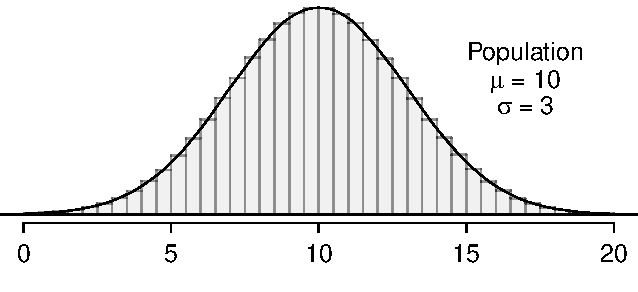
\includegraphics[width=0.55\textwidth]{ch_distributions/figures/eoce/identify_dist_symm_pop/identify_dist_symm_pop.pdf} \\
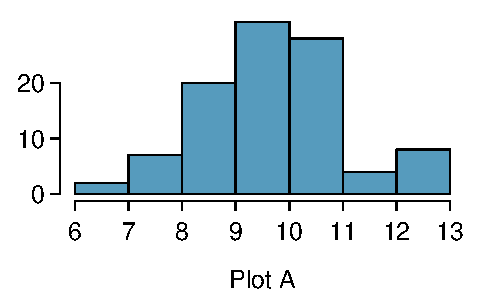
\includegraphics[width=0.325\textwidth]{ch_distributions/figures/eoce/identify_dist_symm_pop/identify_dist_symm_sampling_n5.pdf}
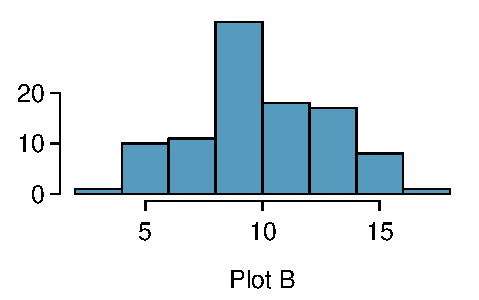
\includegraphics[width=0.325\textwidth]{ch_distributions/figures/eoce/identify_dist_symm_pop/identify_dist_symm_samp.pdf}
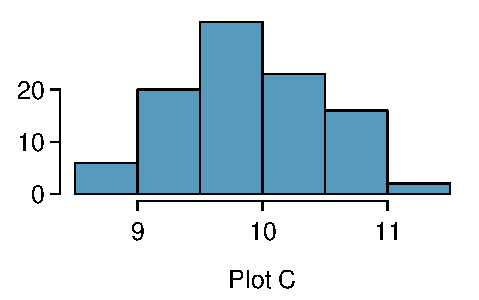
\includegraphics[width=0.325\textwidth]{ch_distributions/figures/eoce/identify_dist_symm_pop/identify_dist_symm_sampling_n25.pdf}
\end{center}
}{}

% 12 - identify_dist_ls_pop

\eoce{\qt{Identify distributions, Part II\label{identify_dist_ls_pop}} Four plots are presented below. The plot at 
the top is a distribution for a population. The mean is 60 and the standard 
deviation is 18. Also shown below is a distribution of (1) a single random 
sample of 500 values from this population, (2) a distribution of 500 sample 
means from random samples of each size 18, and (3) a distribution of 500 sample 
means from random samples of each size 81. Determine which plot (A, B, or C) is 
which and explain your reasoning.
\begin{center}
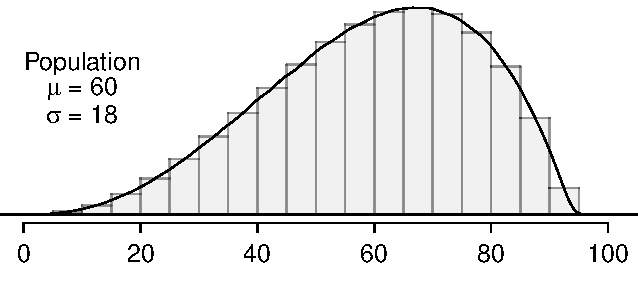
\includegraphics[width=0.55\textwidth]{ch_distributions/figures/eoce/identify_dist_ls_pop/identify_dist_ls_pop.pdf}
\end{center}
\begin{center}
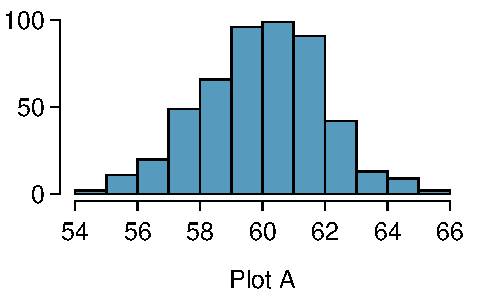
\includegraphics[width=0.325\textwidth]{ch_distributions/figures/eoce/identify_dist_ls_pop/identify_dist_ls_sampling_n81.pdf}
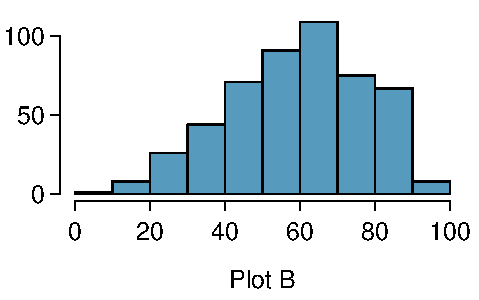
\includegraphics[width=0.325\textwidth]{ch_distributions/figures/eoce/identify_dist_ls_pop/identify_dist_ls_samp.pdf}
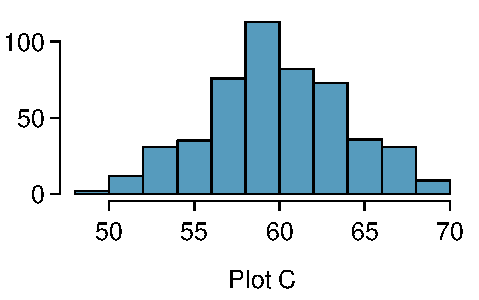
\includegraphics[width=0.325\textwidth]{ch_distributions/figures/eoce/identify_dist_ls_pop/identify_dist_ls_sampling_n18.pdf}
\end{center}
}{}

% 13 - penny_weights

\eoce{\qt{Weights of pennies\label{penny_weights}} The distribution of weights of 
United States pennies is approximately normal with a mean of 2.5 grams and a 
standard deviation of 0.03 grams.
\begin{parts}
\item What is the probability that a randomly chosen penny weighs less than 2.4 
grams?
\item Describe the sampling distribution of the mean weight of 10 randomly 
chosen pennies.
\item What is the probability that the mean weight of 10 pennies is less than 
2.4 grams?
\item Sketch the two distributions (population and sampling) on the same scale.
\item Could you estimate the probabilities from (a) and (c) if the weights of pennies had a skewed distribution?
\end{parts}
}{}

% 14 - cflbs

\eoce{\qt{CFLBs\label{cflbs}} A manufacturer of compact fluorescent light bulbs advertises 
that the distribution of the lifespans of these light bulbs is nearly normal with 
a mean of 9,000 hours and a standard deviation of 1,000 hours.
\begin{parts}
\item What is the probability that a randomly chosen light bulb lasts more than 
10,500 hours?
\item Describe the distribution of the mean lifespan of 15 light bulbs. 
\item What is the probability that the mean lifespan of 15 randomly chosen light 
bulbs is more than 10,500 hours?
\item Sketch the two distributions (population and sampling) on the same scale.
\item Could you estimate the probabilities from parts~(a) and~(c) if the 
lifespans of light bulbs had a skewed distribution?
\end{parts}
}{}

% 15 - songs_on_ipod

\eoce{\qt{Songs on an iPod\label{songs_on_ipod}} Suppose an iPod has 3,000 songs. The 
histogram below shows the distribution of the lengths of these songs. We also 
know that, for this iPod, the mean length is 3.45 minutes and the standard 
deviation is 1.63 minutes.
\begin{center}
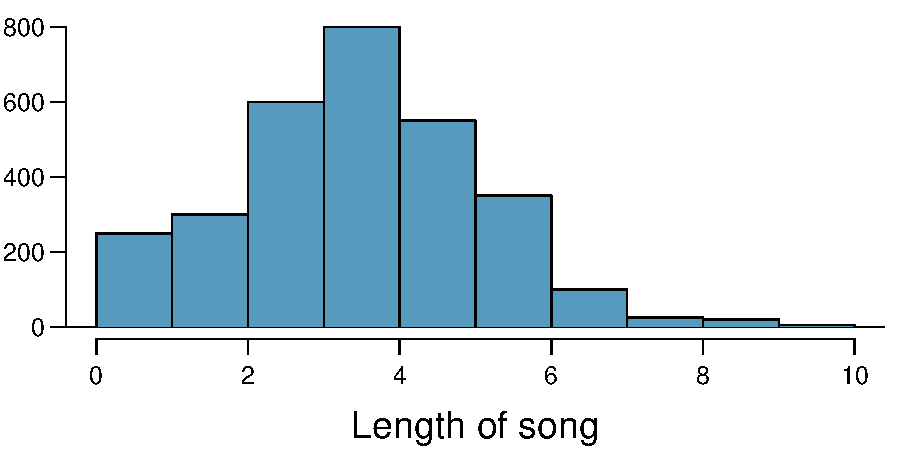
\includegraphics[width=0.5\textwidth]{ch_distributions/figures/eoce/songs_on_ipod/songs_on_ipod_pop_hist.pdf}
\end{center}
\begin{parts}
\item Calculate the probability that a randomly selected song lasts more than 5 
minutes.
\item You are about to go for an hour run and you make a random playlist of 15 songs. What is the probability that your playlist lasts for the entire duration 
of your run? \textit{Hint:} If you want the playlist to last 60 minutes, what should be the minimum average length of a song?
\item You are about to take a trip to visit your parents and the drive is 6 hours. You make a random playlist of 100 songs. What is the probability that your playlist lasts the entire drive?
\end{parts}
}{}

% 16 - spray_paint_2

\eoce{\qt{Spray paint, Part II\label{spray_paint_2}} Suppose the area that can be painted using a 
single can of spray paint is slightly variable and follows a nearly normal 
distribution with a mean of 25 square feet and a standard deviation of 3 square 
feet. 
\begin{parts}
\item What is the probability that the area covered by a can of spray paint is 
more than 27 square feet?
\item Suppose you want to spray paint an area of 540 square feet using 20 cans 
of spray paint. On average, how many square feet must each can be able to cover 
to spray paint all 540 square feet?
\item What is the probability that you can cover a 540 square feet area using 20 
cans of spray paint?
\item If the area covered by a can of spray paint had a slightly skewed 
distribution, could you still calculate the probabilities in parts~(a) and~(c) 
using the normal distribution?
\end{parts}
}{}

% 17 - wireless_routers

\eoce{\qt{Wireless routers\label{wireless_routers}} John is shopping for wireless routers and is overwhelmed by the number of available options. In order to get a feel for the average price, he takes a random sample of 75 routers and finds that the average price for this sample is \$75 and the standard deviation is \$25. 
\begin{parts}
\item Based on this information, how much variability should he expect to see in the mean prices of repeated samples, each containing 75 randomly selected wireless routers?
\item A consumer website claims that the average price of routers is \$80. Is a true average of \$80 consistent with John's sample?
\end{parts}
}{}

% 18 - betting_on_dinner_2

\eoce{\qt{Betting on dinner, Part II\label{betting_on_dinner_2}} Exercise~\ref{betting_on_dinner_1} introduces a promotion at a restaurant where prices of menu items are determined randomly following some underlying distribution. We are told that the price of basket of fries is drawn from a normal distribution with mean 6 and standard deviation of 2. You want to get 5 baskets of fries but you only have \$28 in your pocket. What is the probability that you would have enough money to pay for all five baskets of fries?
}{}
}


%______________________________________________
\reviewchapterheader{}

\noindent This chapter began by introducing the idea of sampling distribution.  As with any distribution, we can summarize a sampling distribution with regard to its center, spread, and shape.  A common thread that ran through this chapter is the application of \termni{normal approximation} (introduced in Section~\ref{normalDist}) to different sampling distributions.
\\

\noindent The key steps are included for each of the normal approximation scenarios below.  To verify that the observations can be considered independent verify that you have one of the following: a random process, a random sample with replacement, or a random sample without replacement of less than 10\% of the population.

\begin{enumerate}

\item Normal approximation for the \termni{number of successes} (binomial):  
\\- Verify that observations can be treated as independent and that $np\ge 10$ and $n(1-p)\ge 10$.
\\- Use $\mu_{\scriptscriptstyle{X}} = np$ and $\sigma_{\scriptscriptstyle{X}} = \sqrt{np(1-p)}$ to find the Z-score for the given number of successes.  

\item Normal approximation for a \termni{sample proportion}:  
\\- Verify that observations can be treated as independent and that $np\ge 10$ and $n(1-p)\ge 10$.
\\- Use $\mu_{\hat{p}} = p$ and $\sigma_{\hat{p}} = \sqrt{\frac{p(1-p)}{n}}$ to find the Z-score for the given sample proportion.

\item Normal approximation for \textbf{data}:  (introduced in Section~\ref{normalDist})
\\- Verify that observations can be treated as independent and that population is approximately normal.
\\- Use the given mean $\mu$ and SD $\sigma$ to find the Z-score for the given $x$ value.

\item Normal approximation for a \termsub{sample mean/sum}{sample mean}\index{sample sum|textbf}:  
\\Verify that observations can be treated as independent and that population is approximately normal or that $n\ge 30$.
\\Use $\mu_{\bar{x}}=\mu$ and $\sigma_{\bar{x}}=\frac{\sigma}{\sqrt{n}}$ to find the Z-score for the given/calculated sample mean.

\item In Section \ref{normapproxsumrv}, we saw how to use normal approximation for the \term{sum or difference of two independent random variables}:
\\- Verify that observations can be treated as independent and that each random variable is approximately normal.
\\- Use $E(X+Y)=E(X)+E(Y)$ or $E(X-Y)=E(X)-E(Y)$ and $SD(X+Y)=SD(X-Y)=\sqrt{(SD(X))^2+(SD(Y))^2}$ to find the Z-score for the given sum or difference.

\end{enumerate}


\noindent Cases 3 and 4 apply to \term{numerical} variables, while cases 1 and 2 are for \term{categorical} yes/no variables.  Case 5 applies to both numerical and categorical variables.
\\
\\Note that in the binomial case and in the case of proportions, we never look to see if the \emph{population} is normal.  That would not make sense because the ``population" is simply a bunch of no/yes, 0/1 values and could not possibly be normal.
\\
\\The \term{Central Limit Theorem} is the mathematical rule that ensures that when the sample size is sufficiently large, the sample mean/sum and sample proportion/count will be approximately normal.  
\\
\\
In Sections~\ref{diffofprops} and~\ref{differenceOfTwoMeans}, we applied Case~5 to find the mean and standard deviation for the difference of sample proportions and the difference of sample means.